\documentclass[hidelinks,12pt]{article}
\usepackage[left=0.25cm,top=1cm,right=0.25cm,bottom=1cm]{geometry}
%\usepackage[landscape]{geometry}
\textwidth = 20cm
\hoffset = -1cm
\usepackage[utf8]{inputenc}
\usepackage[spanish,es-tabla, es-lcroman]{babel}
\usepackage[autostyle,spanish=mexican]{csquotes}
\usepackage[tbtags]{amsmath}
\usepackage{nccmath}
\usepackage{amsthm}
\usepackage{amssymb}
\usepackage{mathrsfs}
\usepackage{graphicx}
\usepackage{subfig}
\usepackage{caption}
%\usepackage{subcaption}
\usepackage{standalone}
\usepackage[outdir=./Imagenes/]{epstopdf}
\usepackage{siunitx}
\usepackage{physics}
\usepackage{color}
\usepackage{float}
\usepackage{hyperref}
\usepackage{multicol}
\usepackage{multirow}
%\usepackage{milista}
\usepackage{anyfontsize}
\usepackage{anysize}
%\usepackage{enumerate}
\usepackage[shortlabels]{enumitem}
\usepackage{capt-of}
\usepackage{bm}
\usepackage{mdframed}
\usepackage{relsize}
\usepackage{placeins}
\usepackage{empheq}
\usepackage{cancel}
\usepackage{pdfpages}
\usepackage{wrapfig}
\usepackage[flushleft]{threeparttable}
\usepackage{makecell}
\usepackage{fancyhdr}
\usepackage{tikz}
\usepackage{bigints}
\usepackage{menukeys}
\usepackage{tcolorbox}
\tcbuselibrary{breakable}
\usepackage{scalerel}
\usepackage{pgfplots}
\usepackage{pdflscape}
\pgfplotsset{compat=1.16}
\spanishdecimal{.}
\renewcommand{\baselinestretch}{1.5} 
\renewcommand\labelenumii{\theenumi.{\arabic{enumii}})}

\newcommand{\python}{\texttt{python}}
\newcommand{\textoazul}[1]{\textcolor{blue}{#1}}
\newcommand{\azulfuerte}[1]{\textcolor{blue}{\textbf{#1}}}
\newcommand{\funcionazul}[1]{\textcolor{blue}{\textbf{\texttt{#1}}}}

\newcommand{\pderivada}[1]{\ensuremath{{#1}^{\prime}}}
\newcommand{\sderivada}[1]{\ensuremath{{#1}^{\prime \prime}}}
\newcommand{\tderivada}[1]{\ensuremath{{#1}^{\prime \prime \prime}}}
\newcommand{\nderivada}[2]{\ensuremath{{#1}^{(#2)}}}


\newtheorem{defi}{{\it Definición}}[section]
\newtheorem{teo}{{\it Teorema}}[section]
\newtheorem{ejemplo}{{\it Ejemplo}}[section]
\newtheorem{propiedad}{{\it Propiedad}}[section]
\newtheorem{lema}{{\it Lema}}[section]
\newtheorem{cor}{Corolario}
\newtheorem{ejer}{Ejercicio}[section]

\newlist{milista}{enumerate}{2}
\setlist[milista,1]{label=\arabic*)}
\setlist[milista,2]{label=\arabic{milistai}.\arabic*)}
\newlength{\depthofsumsign}
\setlength{\depthofsumsign}{\depthof{$\sum$}}
\newcommand{\nsum}[1][1.4]{% only for \displaystyle
    \mathop{%
        \raisebox
            {-#1\depthofsumsign+1\depthofsumsign}
            {\scalebox
                {#1}
                {$\displaystyle\sum$}%
            }
    }
}
\def\scaleint#1{\vcenter{\hbox{\scaleto[3ex]{\displaystyle\int}{#1}}}}
\def\scaleoint#1{\vcenter{\hbox{\scaleto[3ex]{\displaystyle\oint}{#1}}}}
\def\scaleiiint#1{\vcenter{\hbox{\scaleto[3ex]{\displaystyle\iiint}{#1}}}}
\def\bs{\mkern-12mu}

\newcommand{\Cancel}[2][black]{{\color{#1}\cancel{\color{black}#2}}}


\usepackage{minted}

\author{M. en C. Gustavo Contreras Mayén. \texttt{gux7avo@ciencias.unam.mx}}
\title{Evaluación del Examen Final \\ {\large Curso Física Computacional}}
\date{ }
\begin{document}

\maketitle
\fontsize{14}{14}\selectfont

\Large{Mayorquin Galicia Antonio.}

\section{Problema 1.}

\begin{enumerate}
\item En tu función \texttt{raizSecante} habría que aclarar bien los elementos que se deben de implementar para el método de la secante:
\begin{enumerate}
\item En español no se dice: \enquote{Valor a empezar a buscar la raíz}.
\item Como tampoco se escribe \enquote{Tolerancia entre la cercanez ...}
\item Esto pone en evidencia que aunque hiciste alguna revisión para el método, el traductor de idioma no aclara bien lo que presentas.
\end{enumerate}
El método de la secante requiere de dos valores $x_{0}$ y $x_{1}$ que son las aproximaciones de la raíz, para tender precisamente una recta secante, de esta manera se va iterando hasta que se cumpla la tolerancia esteblecida.
\item Revisa que:
\begin{minted}{python}
xn_1 = x0
fn_1 = f(xn_1)
xn = xn_1 + dx0
fn = (xn) 
\end{minted}
Parecería que tienes un error por que \texttt{fn} debe de ser la función evaluada en el segundo punto de aproximación, que si bien lo ocupas, el valor que usas $0.1$, ¿te permitiría identificar una raíz?
\item Para la segunda raíz reportas un valor de $7.7056$, cuando se espera $7.70595$. La segunda aproximación que necesita el método de la secante es \enquote{pequeña} aunque el valor de tolerancia que ocupas es razonable, no se identifica el por qué usaste ese valor y no otro.
\item \textbf{Calificación: 0.9 puntos}
\end{enumerate}

\section{Problema 2.}

\begin{enumerate}
\item En tu elección del método de integración, argumentas que el método de Simpson 1/3 \emph{es el más reconocido}, que si bien es cierto, también mencionamos que el método de integración de Romberg es más eficiente, por lo que hay que elegir el método más pertinente, como recordarás, el método de Romberg prácticamente abate el error asociado en la integración.
\item Al tener una suma con dos sumandos, recuerda que también hay un error asociado a esa operación.
\item \textbf{Calificación: 0.9 puntos}
\end{enumerate}

\section{Problema 3.}

\begin{enumerate}
\item Como en el ejercicio anterior, te decides por un método conocido, cuando lo que se busca es la eficiencia.
\item Aunque haces lo necesario para el par de métodos que propones, el trabajo se reduce si eliges el método de Romberg.
\item \textbf{Calificación: 0.9 puntos}
\end{enumerate}

\section{Problema 4.}

\begin{enumerate}
\item Con respecto a \enquote{identificamos que la definición de un sistema rigido no es explicitamente  establecido}, te comento que se presentó en clase la definición y se revisaron ejercicios.
\item En la revisión del valor de $h$ mencionas que \enquote{Nuestro h, sea la mitad de la cota máxima ...}, no tienes una cota máxima, sino un valor que si se supera, durante la integración se tendrán resultados no esperados. Cualquier valor por debajo del $h$ calculado está bien, siempre y cuando se mantenga la desigualdad, recuerda que si lo haces más pequeño, se requiere de una mayor número de pasos de integración.
\item Procura que las llamadas de librerías, módulos y funciones estén al inicio del archivo, aunque manejes celdas ya no es necesario volver a llamarlas, esto deja más limpio tu código. Si tienes varias celdas, lo normal es comenzar a ejecutarlas de arriba a abajo, eso te da la garantía de que siempre se ejecutará lo que llames.
\item En la gráfica para el RK no adaptativo, se esperaba que se indicase el paso de integración:
\begin{figure}[H]
    \centering
    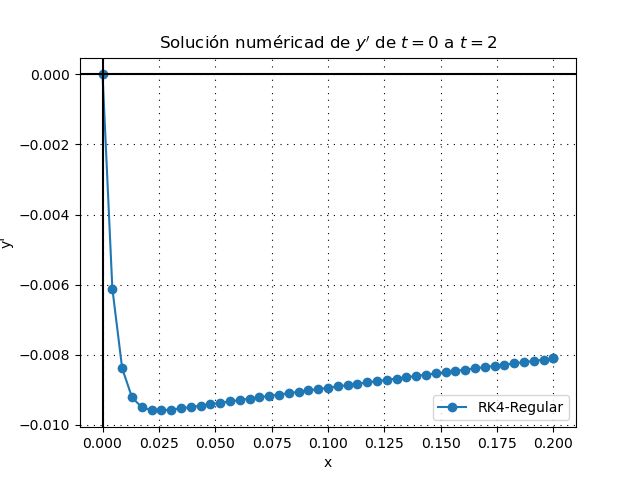
\includegraphics[scale=0.8]{Evidencia_02_04_01_Antonio.png}
    \caption{Es evidente el uso de la $h$ calculada.}
\end{figure}
Mientras que en la gráfica para el RK adaptativo, nuevamente se esperaba visualizar el paso de integración:
\begin{figure}[H]
    \centering
    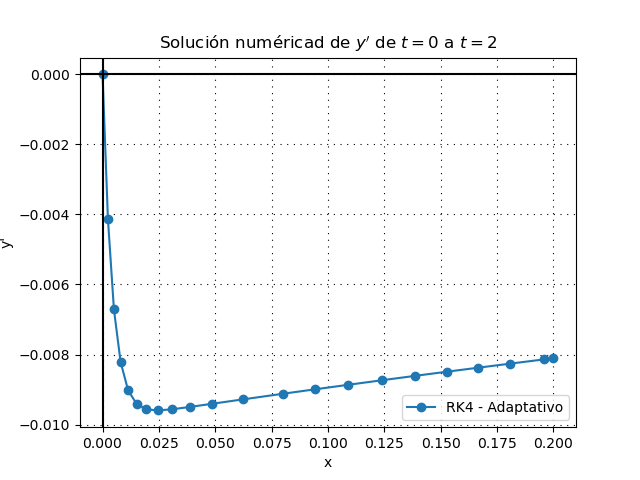
\includegraphics[scale=0.8]{Evidencia_02_04_02_Antonio.png}
    \caption{El método predictor-corrector hace lo suyo y ajusta el valor de $h$.}
\end{figure}
De esta manera, es posible discutir el efecto de $h$ calculada con la segunda técnica. Al superponer las dos gráficas, claramente la solución es única y no se distingue el cálculo de $h$.
\item \textbf{Calificación: 1 punto} Nota: la calificación máxima es de $2$ puntos para este ejercicio.
\end{enumerate}

\section{Problema 5.}

\begin{enumerate}
\item En tu planteamiento inicial para llegar al sistema de ecuaciones algebraicas, tienes que:
\begin{figure}[H]
    \centering
    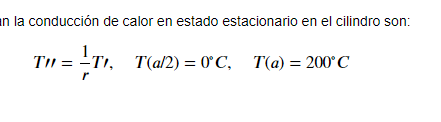
\includegraphics[scale=1]{Evidencia_02_05_00_Antonio.png}
\end{figure}
que no es correcta, ya que en el enunciado el lado derecho de la ED  lleva un signo negativo.

Siendo entonces la expresión correcta:
\begin{align*}
\left( 1 - \dfrac{h}{2 r_{i}} \right) T_{i-1} - 2 T_{i} + \left( 1 + \dfrac{h}{2 r_{i}} \right) T_{i+1} = 0
\end{align*}
\item En tu notebook de Jupyter mencionas que \enquote{... podemos construir nuestra matriz}, pero nunca la presentas, es decir, para pasar al código de la función \texttt{ecuaciones} se debe de saber cómo es el arreglo necesario, ya que eso te permite identificar el tipo de matriz de banda que resulta, esta parte no la discutes ni justificas que entonces al tener un sistema tridiagonal, se van a ocupar las correspondientes funciones que resuelven un sistema en banda.
\item En tu función \texttt{ecuaciones} tienes un comentario en donde muestras en el notebook de Jupyter la ecuacion algebraica para los i-puntos de $[1, m]$, pero en la definición de los vectores columna \texttt{c} y \texttt{e}, inviertes el signo del coeficiente de acuerdo a la expresión que llegaste, y no se aclara el por qué cambias el signo! 
\item Al dejar los signos de acuerdo a tu expresión, la solución claramente no es la esperada:
\begin{figure}[H]
    \centering
    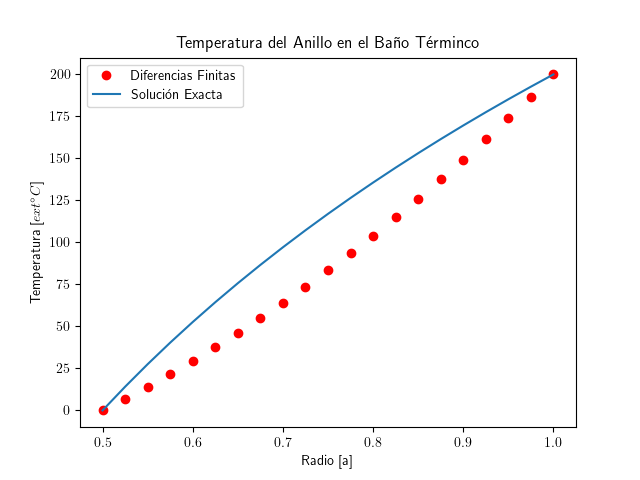
\includegraphics[scale=0.8]{Evidencia_02_05_00b_Antonio.png}
\end{figure}
aunque en tu gráfica el resultado que se muestra, es el correspondiente al problema de la ecuación de calor, que claramente coincide con la solución analítica del problema.
\item El correcto signo en la expresión algebraica que obtuviste te lleva a un resultado distinto.
\item \textbf{Calificación: 0.5 puntos}
\end{enumerate}

\section{Problema 6.}

\begin{enumerate}
\item En el primer desarrollo por mallas con la ley de Kirchhoff para la corriente, llegas a las expresiones correctas.
\item Luego donde mencionas \enquote{Al diferenciar con respecto al tiempo...} supongo que haces $\dv*{q_{i}}{t}$ lo que te dejaría para cada ecuación, un término $\displaystyle C L \dv[2]{i_{i}}{t}$, pero sigues indicando las cargas.
\item En el primer renglón donde tienes:
\begin{align*}
q_{1} + 2(q_{1} - q_{2}) = 3 q_{1} - 2 q_{2} \neq - 3 q_{1} + 2 q_{2} \hspace{0.5cm} \text{que tu calculaste!}  
\end{align*}
\item En cada uno de los siguientes tres renglones tienes valores que no corresponden a las cargas, el álgebra pone en evidencia que llegas a una matriz de coeficientes que no es la correspondiente. Siendo la correcta:
\begin{align*}
\begin{bmatrix}
3 & -2 & 0 & 0 \\
-2 & 5 & -3 & 0 \\
0 & -3 & 7 & -4 \\
0 & 0 & -4 & 9
\end{bmatrix}
\end{align*}
\item En el resultado que obtuviste de los eigenvalores, por definición esos valores no tienen sentido físico, que de antemano ya te hubiera alertado para revisar que algo sucedió durante el planteamiento del problema.
\item Aunque el procedimiento que sigues es el indicado, no nos lleva a un resultado consistente por que de inicio, el sistema que recuperas no es el del fenómeno físico.
\item \textbf{Calificación: 0.4 puntos.}
\end{enumerate}

\section{Problema 7.}

\begin{enumerate}
\item En este ejercicio si presentas el sistema con matrices que se obtiene del circuito eléctrico.
\item Hay un detalle en tu sistema, ya que la matriz de coeficientes que va al lado izquierdo de la expresión, es la que corresponde a los coeficientes de $\dv*[2]{u_{i}}{t}$, haciendo $\lambda = (\omega^{2} L C)^{-1}$, entonces te queda el sistema:
\begin{align*}
\begin{bmatrix}
2 & -1 & 0 & 0 \\
-1 & 2 & -1 & 0 \\
0 & - 1 & 2 & -1 \\
0 & 0 & -1 & 2
\end{bmatrix}
\begin{bmatrix}
u_{1} \\
u_{2} \\
u_{3} \\
u_{4}
\end{bmatrix} = 
\lambda 
\begin{bmatrix}
1 & 0 & 0 & 0 \\
0 & 2 & 0 & 0 \\
0 & 0 & 3 & 0 \\
0 & 0 & 0 & 4
\end{bmatrix}
\begin{bmatrix}
u_{1} \\
u_{2} \\
u_{3} \\
u_{4}
\end{bmatrix}
\end{align*}
\item Si en el desarrollo llegas a las matrices, ¿por qué las multiplicas por $-1$ en el código? Eso te lleva a otro resultado!
\item Deberías de explicar en qué consiste el \enquote{método de housedorf}, que no vimos en clase. Vimos un método que se llama \textbf{método de Householder}, que entiendo es otro al que refieres, este tipo de situaciones no deben de presentarse en un examen final!
\item El resultado al que llegas: eigenvalores negativos, nuevamente es un gran aviso para identificar que algo no está bien!
\item Las frecuencias angulares correctas son:
\begin{align*}
[0.64711605 \quad 2.61701309 \quad 0.96278991 \quad 1.34369599]
\end{align*}
en unidades de $\sqrt{L C}$.
\item \textbf{Calificación: 0.4 puntos}
\end{enumerate}

\section{Problema 8.}

\begin{enumerate}
\item Tu desarrollo comienza bien, recuerda que si bien las expresiones con las que se apoya el enunciado pueden tener alguna imprecisión, no quiere decir que el alumno no haga el estudio del problema y corregir entonces, el error. En este caso, siendo un problema de mecánica clásica, para un alumno del sexto semestre es posible hacer ese estudio sin contratiempo.
\item Es recomendable hacer toda la descripción de tareas o procedimientos que vas a ocupar, si bien llegas a la definición de la forma estándar para resolver el problema, ya luego no se sabe qué es lo que vas a hacer, solo llegando al código es donde se encuentra el camino que seguiste.
\item En tu función \texttt{minNlamdeH} no es necesario el manejo que propones de usar una matriz $\vb{A}$, ya que desde el desarrollo a mano sabes que es una matriz tridiagonal, de la forma $\vb{A} = [\vb{c} \backslash \vb{d} \backslash \vb{c}]$, siendo el manejo de un vector columna el más apropiado. 
\item Tu paso a la forma estándar no es el correspondiente.
\item En clase se presentó un método para obtener los eigenvalores más pequeños: \textbf{Método de la potencia inversa (normal o con desplazamiento)}, que es el necesario para responder el ejercicio, la función \texttt{sort} ordena los elementos de un objeto en cierto sentido, pero no son procedimientos equivalentes. En las notas del Tema 4 se presentaron las técnicas y se resolvieron ejercicios.
\item Según tu resultado, las dos frecuencias angulares corresponden a un mismo eigenvalor, que nos diría que tenemos entonces un sistema degenerado, pero claramente no es lo que presenta el sistema de masas-resorte. Nuevamente llegas a un valor que te avisa claramente que no hay concordancia con la física involucrada.
\item Faltó también calcular el desplazamiento de las masas para cada eigenvalor.
\item Las $N = 2$ frecuencias angulares más pequeñas son:
\begin{align*}
[74.268887 \quad 215.306539 ]
\end{align*}
\item \textbf{Calificación: 0 puntos.}
\end{enumerate}

\end{document}